\fancyhead[RE]{\textit{List of Released Softwares}}
\fancyhead[LO]{\textit{List of Released Softwares}}

\section*{Software released with the \texttt{dict2vec} publication:}
  \url{https://github.com/tca19/dict2vec}

  \begin{figure}[h]
    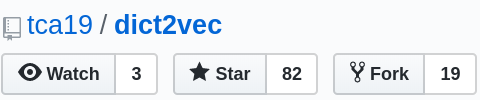
\includegraphics[width=0.5\textwidth]{ch09-d2v-repo-stats}
  \end{figure}

  \noindent This repository contains:

  \begin{itemize}
    \item scripts to automatically download the webpages of 4 different English
      dictionaries (Cambridge, Oxford, Collins and dictionary.com), parse their
      content and extract word definitions;
    \item scripts to generate strong and weak pairs from the downloaded
      definitions;
    \item script to download the latest Wikipedia dump and generate the 50M
      tokens, the 200M tokens and the full Wikipedia training corpora;
    \item source code to train the \texttt{dict2vec} model and learn word
      embeddings using the pairs generated from the definitions of dictionaries;
    \item source code to evaluate word embeddings (learned with
      \texttt{dict2vec} or with any other common method) on a word semantic
      similarity task on thirteen evaluation datasets;
    \item links to download pre-trained vectors learned with the
      \texttt{dict2vec} model on a 50M tokens, a 200M tokens and a full
      Wikipedia corpora.
  \end{itemize}

\section*{Software released with the \texttt{NLB} publication:}
  \url{https://github.com/tca19/near-lossless-binarization}

  \begin{figure}[h]
    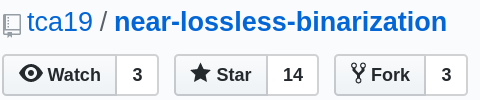
\includegraphics[width=0.5\textwidth]{ch09-nlb-repo-stats}
  \end{figure}

  \noindent This repository contains:

  \begin{itemize}
    \item source code to train the \texttt{NLB} autoencoder to transform any
      pre-trained real-valued word embeddings into binary vectors;
    \item source code to evaluate binary word vectors on a word semantic
      similarity task on five evaluation datasets;
    \item source code to find the $K$ closest words of a query word from the
      binary word vectors.
  \end{itemize}
